% !TeX root = ../Book2.tex
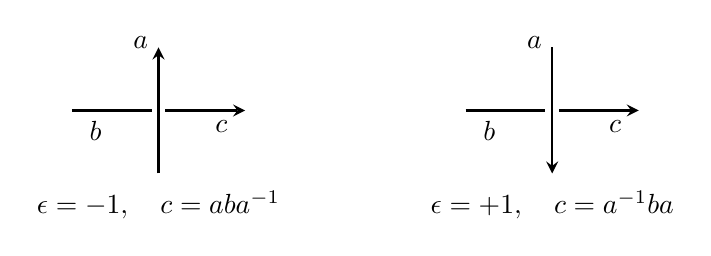
\begin{tikzpicture}[line width=.9pt,>=stealth,over/.style={preaction={draw=white,line width=5pt}}]
	\begin{scope}
		\draw[->] (-1.1,0)--(1.1,0);
		\draw[over,->] (0,-.8)--(0,.8);
		\node[above left] at (0,.65) {\(a\)};
		\node[below] at (-.8,0) {\(b\)};
		\node[below] at (.8,0) {\(c\)};
		\node at (0,-1.2) {\(\epsilon=-1,\quad c=aba^{-1}\)};
	\end{scope}
	\begin{scope}[xshift=5cm]
		\draw[->] (-1.1,0)--(1.1,0);
		\draw[over,->] (0,.8)--(0,-.8);
		\node[above left] at (0,.65) {\(a\)};
		\node[below] at (-.8,0) {\(b\)};
		\node[below] at (.8,0) {\(c\)};
		\node at (0,-1.2) {\(\epsilon=+1,\quad c=a^{-1}ba\)};
	\end{scope}
\end{tikzpicture}
